% Copyright 2006 by Till Tantau
%
% This file may be distributed and/or modified
%
% 1. under the LaTeX Project Public License and/or
% 2. under the GNU Free Documentation License.
%
% See the file doc/generic/pgf/licenses/LICENSE for more details.


% \section{Guidelines on Graphics}
\section{绘图指导}

\bohs

% The present section is not about \pgfname\ or \tikzname, but about
% general guidelines and principles concerning the creation of
% graphics for scientific presentations, papers, and books.
这一节不是讲 \pgfname\ 和 \tikzname\ 的,而是讲在科学报告、论文和书籍中绘制图形时,通用的指导和原则。

% The guidelines in this section come from different sources. Many of
% them are just what I would like to claim is ``common sense,'' some
% reflect my personal experience (though, hopefully, not my personal
% preferences), some come from books (the bibliography is still missing,
% sorry) on graphic design and typography.
% The most influential source  are the brilliant books
% by Edward Tufte. While I do not agree with everything written in these
% books, many of Tufte's arguments are so convincing that I decided to
% repeat them in the following guidelines.
本节的指导源自不同的地方,我想声明的内容,大多都只是“常识”,一些基于我的个人经历(当然,我希望并不只是我个人的偏好),一些来自图形设计和排版的书籍(还没写参考文献,见谅)。

% The first thing you should ask yourself when someone presents a bunch of
% guidelines is: Should I really follow these guidelines? This is an
% important question, because there are good reasons not to follow
% general guidelines.  The person who set up the guidelines may have had other
% objectives than you do. For example, a guideline might say ``use the
% color red for emphasis.'' While this guideline makes perfect sense
% for, say, a presentation using a projector, red ``color'' has the
% \emph{opposite} effect of ``emphasis'' when printed using a
% black-and-white printer. Guidelines were almost always set up to
% address a specific situation. If you are not in this situation,
% following a guideline can do more harm than good.
当有人给你列出一堆指导时,你首先得问自己:我真的应该遵循这些指导吗?
这是个重要的问题,因为有很多好理由不去遵循这些通用的指导。
给出这些指导的人,目标可能和你的并不一致。
比如说,某条指导可能写“用红色来强调”,这可能非常适合用投影仪做的报告,但是对于黑白打印的内容来说,红色可能就起了\emph{相反的}效果。
指导几乎总是用于处理特定的情况,在错误的情况下遵守它只会弊大于利。

% The second thing you should be aware of is the basic rule of
% typography is: ``Every rule can be broken, as long as you are
% \emph{aware}  that you are breaking a rule.'' This rule also applies
% to graphics. Phrased differently, the basic rule states: ``The only
% mistakes in typography are things done in ignorance.''  When you are
% aware of a rule and when you decide that breaking the rule has a
% desirable effect, break the rule.
关于排版的基本规则,你要知道的第二件事是:“每一条规则都可以打破,只要你确实“意识到”你在打破某条规则。”
这条规则也适用于绘图。
上面那句话换个说法,就是:“排版时唯一的错误,就是对发生的事一无所知。”
如果你想打破一条规则并且清楚后果,那么打破它。

\eohs


% \subsection{Planning the Time Needed for the Creation of Graphics}
\subsection{规划绘图用时}

\bohs

% When you create a paper with numerous graphics, the time needed to
% create these graphics becomes an important factor. How much time
% should you calculate for the creation of graphics?
如果你要写一篇图很多的文章,那么一个重要的因素是,画这些图要花多久。
你怎样计算绘图所需的时间呢?

% As a general rule, assume that a graphic will need as much time to
% create as would a text of the same length. For example, when I
% write a paper, I need about one hour per page for
% the first draft. Later, I need between two and four hours per page
% for revisions. Thus, I expect to need about half an hour for the
% creation of \emph{a first draft} of a half page graphic. Later on, I
% expect another one to two hours before the final graphic is finished.
我们假设,画一张图花费的时间,等于写同样篇幅的文字。
比如我写文章,初稿可能一页一小时,到后面修改时,每页可能需要两到四小时。
那么,要画半页左右的图,\emph{初稿}我预计需要半个小时,后面还需要一到两小时,完成最终的图。

% In many publications, even in good journals, the authors and editors
% have obviously invested a lot of time on the text, but seem to
% have spend about five minutes to create all of the
% graphics. Graphics often seem to have been added as an
% ``afterthought'' or look like a screen shot of whatever the authors's
% statistical software shows them. As will be argued later on, the
% graphics that programs like \textsc{gnuplot} produce by default are of
% poor quality.
在许多出版物甚至是优秀的期刊中,作者和编辑明显在文字上花了很多工夫,但是似乎只花了五分钟就画好了所有图。
通常这些图好像就是“后加上的”,或者只是统计软件的截图。
正如后面会讨论的,像 \textsc{gnuplot} 这种软件默认画出来的图,质量并不高。

% Creating informative graphics that help the reader and that fit
% together with the main text is a difficult, lengthy process.
结合文字绘制信息图,从而帮助读者理解,是一个困难而漫长的过程。

\eohs

\begin{itemize}
\item
  % Treat graphics as first-class citizens of your papers. They deserve
  % as much time and energy as the text does.
  % Indeed, the creation of graphics might deserve \emph{even more} time
  % than the writing of the main text since more attention will be paid
  % to the graphics and they will be looked at first.
  把图形作为你文章的一等公民。图形值得花费同文字相等的时间和精力。
  事实上,相比文字,绘图可能值得投入\emph{更多的}时间,因为人们第一眼看到的就是图形,也更关注图形。
\item
  % Plan as much time for the creation and revision of a graphic as you
  % would plan for text of the same size.
  给图形的绘制和修改规划尽可能多的时间,就像对待同等篇幅的文字一样。
\item
  % Difficult graphics with a high information density may require even
  % more time.
  信息量大的困难的图形,可能需要更多的时间。
\item
  % Very simple graphics will require less time, but most likely you do
  % not want to have ``very simple graphics'' in your paper, anyway;
  % just as you would not like to have a ``very simple text'' of the
  % same size.
  简单的图形需要更少的时间,但是无论如何,很可能你并不想在文章里放“非常简单的图”,就像你不想在文章中写同等篇幅“非常简单的文字”一样。
\end{itemize}


% \subsection{Workflow for Creating a Graphic}
\subsection{绘图的工作流程}

\bohs

% When you write a (scientific) paper, you will most likely follow the
% following pattern: You have some results/ideas that you would
% like to report about. The creation of the paper will typically start
% with compiling a rough outline. Then, the different sections are
% filled with text to create a first draft. This draft is then revised
% repeatedly until, often after substantial revision, a final paper
% results. In a good journal paper there is typically not be a single
% sentence that has survived unmodified from the first draft.
你写一篇(科学)文章,通常会遵循下面的模式:
你有一些结果或者想法要阐述。写文章时一般会先列一个粗糙的大纲,然后分别写各个章节,得到初稿。在成稿写好前,一般要不停地大量地修改。
一篇好的期刊文章,初稿里几乎没有一句到最后还没改过的。

% Creating a graphics follows the same pattern:
绘图也遵循相同的模式:

\eohs

\begin{itemize}
\item
  % Decide on what the graphic should communicate. Make this a conscious
  % decision, that is, determine ``What is the graphic supposed to tell
  % the reader?''
  决定图形想要表达什么。一定要有意识地思考,“图形应该告诉读者什么?”
\item
  % Create an ``outline,'' that is, the rough overall ``shape'' of the
  % graphic, containing the most crucial elements. Often, it is
  % useful to do this using pencil and paper.
  列一个“大纲”,也就是图形整体的大致“轮廓”,包含最重要的元素。
  在这一步,笔纸一般很有帮助。
\item
  % Fill out the finer details of the graphic to create a first
  % draft.
  补充和完善图形的细节,得到初稿。
\item
  % Revise the graphic repeatedly along with the rest of the paper.
  根据文章内容,不断修改图形。
\end{itemize}


% \subsection{Linking Graphics With the Main Text}
\subsection{关联图文内容}

\bohs

% Graphics can be placed at different places in a text. Either, they can
% be inlined, meaning they are somewhere ``in the middle of the text''
% or they can be placed in stand-alone ``figures.'' Since printers (the
% people) like to have their pages ``filled,'' (both for aesthetic and
% economic reasons) stand-alone figures may traditionally be placed on
% pages in the document far away from the main text that refers to
% them. \LaTeX\ and \TeX\ tend to encourage this ``drifting away'' of
% graphics for technical reasons.
图形可以置于文本中的不同位置。既可以插在行内,也就是“文字中间”,也可以放在单独的“图片”中。
由于印刷者(也就是人们)喜欢将页面“填满”(同时出于美学和经济的考虑),因此独立的图片通常会放到离相关文字很远的地方。
基于技术原因,\LaTeX\ 和 \TeX\ 倾向于鼓励图形的这种“游离”形式。

% When a graphic is inlined, it will more or less automatically be
% linked with the main text in the sense that the labels of the graphic
% will be implicitly explained by the surrounding text. Also, the main
% text will typically make it clear what the graphic is about and what
% is shown.
插在行内的图形,或多或少和正文有些关联,因为周围的文字间接地解释了图形的标签,
并且通常正文也会阐明这个图形和什么相关,展示了什么。

% Quite differently, a stand-alone figure will often be viewed at a time
% when the main text that this graphic belongs to either has not yet
% been read or has been read some time ago. For this reason, you should
% follow the following guidelines when creating stand-alone figures:
独立的图片则大不相同,读者在看到它们的时候,也许还没读到与之相关的文字,或者已经读过很久了。
因此,如果你要绘制独立的图片,应该遵循如下指导:

\eohs

\begin{itemize}
\item
  % Stand-alone figures should have a caption than should make them
  % ``understandable by themselves.''
  独立的图片应当有一个标题,并且“顾名即可思义”。

  % For example, suppose a graphic shows an example of the different
  % stages of a quicksort algorithm. Then the figure's caption should,
  % at the very least, inform the reader that ``The figure shows the
  % different stages of the quicksort algorithm introduced on page
  % xyz.'' and not just ``Quicksort algorithm.''
  比方说,假设一张图展示了快排算法的不同阶段,那么图片的标题至少应当告诉读者,“该图展示了快排算法的不同阶段,如 xyz 页所述”,而不仅仅是“快排算法”。
\item
  % A good caption adds as much context information as possible. For
  % example, you could say: ``The figure shows the different stages of
  % the quicksort algorithm introduced on page xyz. In the first line,
  % the pivot element 5 is chosen. This causes\dots'' While this
  % information can also be given in the main text, putting it in the
  % caption will ensure that the context is kept. Do not feel afraid of
  % a 5-line caption. (Your editor may hate you for this. Consider
  % hating them back.)
  好的标题会加上尽可能多的上下文信息。
  比如你会写:“该图展示了快排算法的不同阶段,如 xyz 页所述。在第一行中,选择基准元素 5,这会造成 \dots”
  这些信息当然也可以在正文中写出,但是放在标题里保证了上下文。
  不要害怕写一个长达五行的标题。(你的编辑可能会因此讨厌你,你可以把讨厌反弹回去。)
\item
  % Reference the graphic in your main text as in ``For an example of
  % quicksort `in action,' see Figure~2.1 on page xyz.''
  在正文中,你可以这样引用图片:“有一个快排的‘实际’例子,见第 xyz 页的图 2.1。”
\item
  % Most books on style and typography recommend that you do not use
  % abbreviations as in ``Fig.~2.1'' but write ``Figure 2.1.''
  很多讲样式和排版的书,会建议你不要缩写成“Fig.~2.1”,而是应该写“Figure 2.1”。

  % The main argument against abbreviations is that ``a period is too
  % valuable to waste it on an abbreviation.'' The idea is that a period
  % will make the reader assume that the sentence ends after ``Fig'' and
  % it takes a ``conscious backtracking'' to realize that the sentence
  % did not end after all.
  反对缩写的主要论据是,“不应在缩写这种地方浪费句点的价值”。
  意思是,句点会让读者以为句子结束于“Fig”,并且需要“有意识的回溯”,才能发现句子根本没有结束。

  % The argument in favor of abbreviations is that they save space.
  支持缩写的论据是,节省空间。

  % Personally, I am not really convinced by either argument. On the one
  % hand, I have not yet seen any hard evidence that abbreviations slow
  % readers down. On the other hand,  abbreviating all ``Figure'' by
  % ``Fig.''\ is most unlikely to save even a single line in  most
  % documents. I avoid abbreviations.
  我个人并不信服任何一种论据。
  一方面,我还没见过有力的证据,表明缩写会降低阅读速度;另一方面,在大多数文章中,如果将所有“Figure”缩写成“Fig.”,省下的空间几乎连一行都不到。
  我会避免使用缩写。
\end{itemize}


% \subsection{Consistency Between Graphics and Text}
\subsection{统一图文风格}

\bohs

% Perhaps the most common ``mistake'' people do when creating graphics
% (remember that a ``mistake'' in design is always just ``ignorance'')
% is to have a mismatch between the way their graphics look and the way
% their text looks.
人们在绘图时犯得最多的一个“错误”(记住,设计中的“错误”通常只是“无知”),也许就是图形和文字的式样不搭。

% It is quite common that authors use several different programs for
% creating the graphics of a paper. An author might produce some plots
% using \textsc{gnuplot}, a diagram using \textsc{xfig}, and include an
% |.eps| graphic a coauthor contributed using some unknown program. All
% these graphics will, most likely, use different line widths, different
% fonts, and have different sizes. In addition, authors often use
% options like |[height=5cm]| when including graphics to scale them to
% some ``nice size.''
一个很常见的情况是,文章的配图来自几个不同的程序。
作者可能用 \textsc{gnuplot} 作图,\textsc{xfig} 画图表,以及插入一张 |.eps| 格式的图片(它是合作者画的,不知道用的什么程序)。
这些图很可能用了不同的线宽、字体和尺寸。
此外,作者在插入图片的时候,还经常用 \ltz{[height=5cm]} 这样的选项将图片缩放到“漂亮的尺寸”。

% If the same approach were taken to writing the main text, every
% section would be written in a different font at a different size. In
% some sections all theorems would be underlined, in another they would
% be printed all in uppercase letters, and in another in red. In
% addition, the margins would be different on each page.
% Readers and editors would not tolerate a text if it were written in
% this fashion, but with graphics they often have to.
如果写文字也用这种方法的话,那么就相当于:
不同的章节用不同的字体和字号。
书写定理时,在某些章节中都加了下划线,在另一个章节则全用大写字母,再在另外一个章节用红色字体。
此外,不同页面的边距还不一样。
读者和编辑一定不能忍受这样的文字,但是对于图形他们常常不得不忍受。

% To create consistency between graphics and text, stick to the
% following guidelines:
为了保持图文风格一致,请忠于如下指导:

\eohs

\begin{itemize}
\item
  % Do not scale graphics.
  不要缩放图形。

  % This means that when generating graphics using an external program,
  % create them ``at the right size.''
  意思是说,如果用别的程序画图,那么要输出“正确的尺寸”。
\item
  % Use the same font(s) both in graphics and the body text.
  在图文中使用相同的字体。
\item
  % Use the same line width in text and graphics.
  在图文中使用相同的线宽。

  % The  ``line width'' for normal text is the width of the stem of
  % letters like T{}. For \TeX, this is usually
  % $0.4\,\mathrm{pt}$. However, some journals will not accept graphics
  % with a normal line width below $0.5\,\mathrm{pt}$.
  普通文本的“线宽”是指,T 这样的字母中竖直笔画的宽度。
  在 \TeX\ 中,这个值通常是 $0.4\,\mathrm{pt}$。
  不过有些期刊不接受线宽低于 $0.5\,\mathrm{pt}$ 的图形。
\item
  % When using colors, use a consistent color coding in the text and in
  % graphics. For example, if red is supposed to alert the reader to
  % something in the main text, use red also in graphics for important
  % parts of the graphic. If blue is used for structural elements like
  % headlines and section titles, use blue also for structural elements
  % of your graphic.
  图文中使用统一的颜色。
  比方说,如果正文用红色表示警告,那么在图形中的重要部分也应该用红色;
  如果正文用蓝色表示结构元素,比如大标题和章节标题,那么在图形中也应该用蓝色表示结构元素。

  % However, graphics may also use a logical intrinsic color
  % coding. For example, no matter what colors you normally use, readers
  % will generally assume, say, that the color green as ``positive, go,
  % ok'' and red as ``alert, warning, action.''
  不过,图形也可以用符合内在逻辑的(logical intrinsic)颜色。
  比如无论你正常用什么颜色,读者一般总是会认为,绿色表示“正面的、前进、好”(positive, go, ok),而红色表示“警醒、警告、行动”(alert, warning, action)。
\end{itemize}

\bohs

% Creating consistency when using different graphic programs is almost
% impossible. For this reason, you should consider sticking to a single
% graphics program.
用不同的图形程序绘图,几乎不可能保持风格一致。
因此,你应该考虑忠于一种图形程序。

\eohs

% \subsection{Labels in Graphics}
\subsection{图的标签}

\bohs

% Almost all graphics will contain labels, that is, pieces of text that
% explain parts of the graphics. When placing labels, stick to the
% following guidelines:
几乎所有图形中都有标签,也就是文字片段,用于解释图形中的部分内容。
加标签时,遵照如下指导:

\eohs

\begin{itemize}
\item
  % Follow the rule of consistency when placing labels. You should do
  % so in two ways: First, be consistent with the main text, that is,
  % use the same font as the main text also for labels. Second, be
  % consistent between labels, that is, if you format some labels in
  % some particular way, format all labels in this way.
  放置标签时请保持一致。
  需要做到两点:
  一,标签与正文一致,也就是说,标签应当使用与正文相同的字体。
  二,标签之间一致,也就是说,如果某个标签采用了特定的格式,那么其他标签也应使用同一格式。
\item
  % In addition to using the same fonts in text and graphics, you should
  % also use the same notation. For example, if you write $1/2$ in your
  % main text, also use ``$1/2$'' as labels in graphics, not
  % ``0.5''. A $\pi$ is a ``$\pi$'' and not ``$3.141$''. Finally,
  % $\mathrm e^{-\mathrm i \pi}$ is ``$\mathrm e^{-\mathrm i \pi}$'',
  % not ``$-1$'', let alone ``-1''.
  图文除了字体一致外,还要符号一致。
  比如,如果你在正文中用了 $1/2$,那么图的标签中也应当用“$1/2$”,而不是“0.5”。
  $\pi$ 就是“$\pi$”,而不是“$3.141$”。
  最后,$\mathrm e^{-\mathrm i \pi}$ 就是 “$\mathrm e^{-\mathrm i \pi}$”,而不是“$-1$”,更不是“-1”。
\item
  % Labels should be legible. They should not only have a reasonably
  % large size, they also should not be obscured by lines or other
  % text. This also applies to labels of lines and text \emph{behind} the
  % labels.
  标签要清楚易读。不仅要有合适的大小,还不应被直线或者文字遮挡。这也适用于直线的标签和标签\emph{后面}的文字。
\item
  % Labels should be ``in  place.'' Whenever there is enough space,
  % labels should be placed next to the thing they label. Only if
  % necessary, add a (subdued) line from the label to the labeled
  % object. Try to avoid labels that only reference explanations in
  % external legends. Reader have to jump back and forth between the
  % explanation and the object that is described.
  标签的位置要适当。不管空间是否足够,标签都应当靠近所标的内容。
  只有在必要时,才在标签和所标内容之间加上(柔和的)连接线。
  标签不应单纯指向外部的图例说明,否则读者得在图中内容和外部说明之间来回跳读。
\item
  % Consider subduing ``unimportant'' labels using, for example, a gray
  % color. This will keep the focus on the actual graphic.
  考虑将“不重要的”标签柔和化,比如用灰色,这能让读者更关注对应的图形。
\end{itemize}


% \subsection{Plots and Charts}
\subsection{Plots 和 Charts}

\bohs

% One of the most frequent kind of graphics, especially in scientific
% papers, are \emph{plots}. They come in a large variety, including
% simple line plots, parametric plots, three dimensional plots, pie
% charts, and many more.
最常见的图形,尤其是在科学文章中,就是
它囊括的范围很广,包括简单的折线图、参数方程图、三维图、饼图,等等等等。

% Unfortunately, plots are notoriously hard to get right. Partly, the
% default settings of programs like \textsc{gnuplot} or Excel are to
% blame for this since these programs make it very convenient to create
% bad plots.
不幸的是,众所周知,很难作好图。
部分原因在于,\textsc{gnuplot} 或者 Excel 这类程序的默认设置,很容易就作出糟糕的图。

% The first question you should ask yourself when creating a plot is:
% Are there enough data points to merit a plot? If the answer is ``not
% really,'' use a table.
你在作图时,首先得问自己:
数据点的个数值得作图吗?如果答案是“不太值得”,那么用一张表。

% A typical situation where a plot is unnecessary is when people present
% a few numbers in a bar diagram. Here is a real-life example: At the
% end of a seminar a lecturer asked the participants for feedback. Of
% the 50 participants, 30 returned the feedback form. According to the
% feedback, three participants considered the seminar ``very good,''
% nine considered it  ``good,'' ten ``ok,'' eight ``bad,'' and no one thought
% that the seminar was ``very bad.''
一个典型的没必要作图的例子,就是把几个数画在柱状图中。
这里有个现实的例子:一个研讨会快结束时,演讲者向与会者征询反馈。
有 50 名与会者,收回了 30 份反馈表。
根据反馈,3 人觉得研讨会“很好”,9 人觉得“好”,10 人觉得“还行”,8 人觉得“差”,0 人觉得“很差”。

% A simple way of summing up this information is the following table:
要概括这些信息,一个简单的方法就是下面这张表格:

\eohs

\medskip
% \begin{tabular}{lp{3.75cm}r}
\begin{tabular}{lp{10em}r}
  % \emph{Rating given} & \raggedright\emph{Participants (out of 50) who gave this rating} & \emph{Percentage} \\[1.75em]
  \emph{等级} & \raggedright\emph{评价人数(共计50)} & \emph{百分比} \\[0.5em]
  “很好” & \hfil\hphantom{0}3\hfil & \hphantom{0}6\% \\
  “好” & \hfil\hphantom{0}9\hfil & 18\% \\
  “还行” & \hfil10\hfil & 20\% \\
  “差” & \hfil\hphantom{0}8\hfil & 16\% \\
  “很差” & \hfil\hphantom{0}0\hfil & \hphantom{0}0\% \\[2mm]
  未提交 & \hfil20\hfil & 40\% \\
\end{tabular}

\bigskip

\bohs

% What the lecturer did was to visualize the data using a 3D bar
% diagram. It looked like this (except that in reality the numbers
% where typeset using some extremely low-resolution bitmap font and
% were near-unreadable):
演讲者用三维柱状图将数据可视化出来。
看起来像这样:(不过在实际中,打印数字用的是分辨率极低的位图字体,几乎看不清楚)

\eohs

\bigskip
\par
\begin{tikzpicture}[y=0.03cm,z=3mm]
  \foreach \y in {0,20,40,60,80,100}
    \draw[dashed] (0,\y,0) node[left] {\y} -- (0,\y,1)  -- (6,\y,1);

  \draw (0,0,0) -- (0,100,0)  (0,0,1) -- (0,100,1);
  \draw (0,0,0) -- (6,0,0);

  \foreach \x/\xtext/\height in {1/很好/10,2/好/30,3/还行/33,4/差/27,5/很差/0}
  {
    \draw (\x,0) node[rotate=90,anchor=east] {\xtext};

    \begin{scope}[xshift=\x cm]

    \filldraw[fill=blue!50] (-.3,0,0) rectangle (.3,\height,0);
    \filldraw[fill=blue!30] (.3,0,0) -- (.3,0,1) -- (.3,\height,1) -- (.3,\height,0) --cycle;
    \filldraw[fill=blue!20] (-.3,\height,0) -- (.3,\height,0) --
    (.3,\height,1) -- (-.3,\height,1) --cycle;
    \end{scope}
  }
\end{tikzpicture}
\bigskip

\bohs

% Both the table and the ``plot'' have about the same size. If your first
% thought is ``the graphic looks nicer than the table,'' try to answer
% the following questions based on the information in the table or in
% the graphic:
表格和柱状图大小差不多,如果你第一反应是“柱状图比表格好看多了”,那么请根据表格或者柱状图中的信息,试着回答如下问题:

\eohs

\begin{enumerate}
\item
  % How many participants where there?
  与会者总人数是多少?
\item
  % How many participants returned the feedback form?
  提交反馈表的与会者人数是多少?
\item
  % What percentage of the participants returned the feedback form?
  提交反馈表的与会者百分比是多少?
\item
  % How many participants checked ``very good''?
  选择“很好”的与会者人数是多少?
\item
  % What percentage out of all participants checked ``very good''?
  选择“很好”的与会者占所有与会者的百分比是多少?
\item
  % Did more than a quarter of the participants check ``bad'' or ``very bad''?
  选择“差”或者“很差”的与会者是否超过了四分之一?
\item
  % What percentage of the participants that returned the form checked ``very good''?
  选择“很好”的与会者占提交了反馈表的人的百分比是多少?

\end{enumerate}

\bohs

% Sadly, the graphic does not allow us to answer \emph{a single one of these
%   questions}. The table answers all of them directly, except for the last
% one. In essence, the information density of the graphic is very
% close to zero. The table has a much higher information density; despite
% the fact that it uses quite a lot of white space to present a few numbers.
% Here is the list of things that went wrong with the 3D-bar diagram:
悲伤的是,从柱状图中我们不能回答\emph{上述任何一个问题},而表格则能直接告诉我们所有问题的答案,除了最后一个。
实际上,这张柱状图的信息密度几近于零,而表格的信息密度则远高它,尽管只是为了展示几个数,表格就用了很多空白。
下面是三维柱状图中的一系列错误:
\eohs

\begin{itemize}
\item
  % The whole graphic is dominated by irritating background lines.
  整张图都被恼人的背景线支配了。
\item
  % It is not clear what the numbers at the left mean; presumably
  % percentages, but it might also be the absolute number of
  % participants.
  左侧的数字含义不明,猜测可能是百分比,但也可能是与会者的绝对人数。
\item
  % The labels at the bottom are rotated, making them hard to read.
  底部标签旋转了一个角度,很难读。

  % (In the real presentation that I saw, the text was rendered at a very
  % low resolution with about 10 by 6 pixels per letter with wrong
  % kerning, making the rotated text almost impossible to read.)
  (在我看到的实际展示中,文本分辨率很低,每个字母只有 $10 \times 6$ 个像素,并且字距还有问题,这让旋转后的文字几乎完全没法读。)
\item
  % The third dimension adds complexity to the graphic without adding
  % information.
  第三个维度增加了图的复杂度,但没有提供更多的信息。
\item
  % The three dimensional setup makes it much harder to gauge the height
  % of the bars correctly. Consider the ``bad'' bar. It the number this
  % bar stands for more than 20 or less? While the front of the bar is
  % below the 20 line, the back of the bar (which counts) is above.
  第三个维度影响了对柱形高度的判断。
  看下“差”的那根,它比 20 高还是低?
  柱形的正面比 20 低,背面(真正重要的)比 20 高。
\item
  % It is impossible to tell which  numbers are represented by the
  % bars. Thus, the bars needlessly hide the information these bars are
  % all about.
  几乎不可能说出这些柱形表示的数字,因此,柱形掩盖了想要传递的信息。
\item
  % What do the bar heights add up to? Is it 100\% or 60\%?
  这些柱形的高度总和是多少?是 100\% 还是 60\%?
\item
  % Does the bar for ``very bad'' represent 0 or~1?
  “很差”的那根表示的是 0 还是 1?
\item
  % Why are the bars blue?
  为什么柱形用蓝色?
\end{itemize}

\bohs

% You might argue that in the example the exact numbers are not
% important for the graphic. The important things is the ``message,''
% which is that there are more ``very good'' and ``good'' ratings than
% ``bad'' and ``very bad.'' However, to convey this message either use a
% sentence that says so or use a graphic that conveys this message more
% clearly:
你可能会争辩道,这个例子里,数字是否准确对图形并不重要,
重要的是“信息”,也就是“很好”和“好”的比例高于“差”和“很差”。
然而,想传达这个信息只要一句话,或者像下图这样更清晰地展示出来:

\eohs

\medskip
\par
\begin{tikzpicture}
  \colorlet{good}{green!75!black}
  \colorlet{bad}{red}
  \colorlet{neutral}{black!60}
  \colorlet{none}{white}

  % \node[align=center,text width=3cm]{Ratings given by 50~participants};
  \node[align=center,text width=3cm]{在 50 名与会者中所占比例};

  \begin{scope}[line width=4mm,rotate=270]
    \draw[good]          (-123:2cm) arc (-123:-101:2cm);
    \draw[good!60!white] (-36:2cm) arc (-36:-101:2cm);
    \draw[neutral]       (-36:2cm) arc (-36:36:2cm);
    \draw[bad!60!white]  (36:2cm)  arc (36:93:2cm);

    \newcount\mycount
    \foreach \angle in {0,72,...,3599}
    {
      \mycount=\angle\relax
      \divide\mycount by 10\relax
      \draw[black!15,thick] (\the\mycount:18mm) -- (\the\mycount:22mm);
    }

    \draw (0:2.2cm) node[below] {“还行”: 10 (20\%)};
    \draw (165:2.2cm) node[above] {未提交: 20 (40\%)};
    \draw (-111:2.2cm) node[left] {“很好”: 3 (6\%)};
    \draw (-68:2.2cm) node[left] {“好”: 9 (18\%)};
    \draw (65:2.2cm) node[right] {“差”: 8 (16\%)};
    \draw (93:2.2cm) node[right] {“很差”: 0 (0\%)};
  \end{scope}
  \draw[gray] (0,0) circle (2.2cm) circle (1.8cm);
\end{tikzpicture}

\bigskip

\bohs

% The above graphic has about the same information density as the table
% (about the same size and the same numbers are shown). In addition, one
% can directly ``see'' that there are more good or very good ratings
% than bad ones. One can also ``see'' that the number of people who gave
% no rating at all is not negligible, which is quite common for feedback
% forms.
上图拥有和表格相同的信息密度(尺寸和展示的数字都相同)。
此外,人们可以直接“看到”好的评价多于差的评价。还可以看出,没有评价的人数不能忽略,这在使用反馈表时很常见。

% Charts are not always a good idea. Let us look at an example
% that I redrew from a pie chart in \emph{Die Zeit}, June 4th, 2005:
用图表并不总是好主意。我们来看个例子,这是我从 2005 年 6 月 4 日的德国 \emph{时代周刊} 中选取并且重绘的一张饼图。

\eohs

\bigskip
\par
\begin{tikzpicture}
  \begin{scope}[xscale=3.2,yscale=1.2]

    \sffamily
    \coordinate (right border) at (2.0cm,-1.7cm);
    \coordinate (left border)  at (-2.5cm,2.1cm);

    \fill[black!25] ([xshift=-2mm,yshift=1.1cm]left border) rectangle ([xshift=2mm,yshift=-.3cm]right border);

    \node[below right,text width=10cm,inner sep=0pt] at ([yshift=.9cm,xshift=-1mm]left border)
    % { {\color{black!75} \Large Kohle ist am wichtigsten}\\
      % Energiemix bei der deutschen Stromerzeugung 2004};
    { {\color{black!75} \Large 煤最重要}\\
      2004 年德国发电能源结构};

    \filldraw[draw=gray,fill=white] ([xshift=-1mm]left border) node[below right,black]
      % {\footnotesize Gesamte Netto-Stromerzeugung in Prozent, in
      %   Milliarden Kilowattstunden (Mrd.\ kWh)}
      {\footnotesize 占总体发电量百分比,单位为十亿千瓦时 (Mrd.\ kWh)}
      rectangle ([xshift=1mm]right border);

    % The 3D stuff
    \pgfdeclarehorizontalshading{zeit}{100bp}
    {color(0pt)=(black);
      color(25bp)=(black);
      color(37bp)=(white);
      color(50bp)=(black);
      color(62bp)=(white);
      color(75bp)=(black);
      color(100bp)=(black)}

    \shadedraw[very thin,shading=zeit,yshift=-1.5mm] (0,0) circle (1cm);

    \fill[green!20!gray]   (0,0) -- (90:1cm) arc (90:-5:1cm);
    \fill[white!20!gray]   (0,0) -- (-5:1cm) arc (-5:-105:1cm);
    \fill[orange!20!gray]  (0,0) -- (-105:1cm) arc (-105:-180:1cm);
    \fill[orange!60!white] (0,0) -- (180:1cm) arc (180:150:1cm);
    \fill[black!75!white]  (0,0) -- (150:1cm) arc (150:145:1cm);
    \fill[blue!90!white]   (0,0) -- (145:1cm) arc (145:135:1cm);
    \fill[blue!50!white]   (0,0) -- (135:1cm) arc (135:92:1cm);
    \fill[yellow!50!black] (0,0) -- (92:1cm) arc (92:90:1cm);

    \begin{scope}[very thin]
      \draw (0,0) -- (90:1cm);
      \draw (0,0) -- (-5:1cm);
      \draw (0,0) -- (-105:1cm);
      \draw (0,0) -- (-180:1cm);
      \draw (0,0) -- (150:1cm);
      \draw (0,0) -- (145:1cm);
      \draw (0,0) -- (135:1cm);
      \draw (0,0) -- (92:1cm);

      \draw(0,0) circle (1cm);
    \end{scope}

    \node (Regenerative)   at (115:.75cm)  {\bfseries 9,4\%};
    \node (Kernenergie)    at (30:.5cm)   {\bfseries 27,8\%};
    \node (Braunkohle)     at (-45:.6cm)  {\bfseries 25,6\%};
    \node (Steinkohle)     at (-135:.6cm) {\bfseries 22,3\%};
    \node (Erdgas)         at (168:.75cm) {\bfseries 10,4\%};
    \coordinate (Mineral)  at (147:.9cm);
    \coordinate (Sonstige) at (140:.9cm);

    \small
    \draw (Regenerative.north) |- ([yshift=.25cm]Regenerative.north -| right border) coordinate (Regenerative label);
    \draw (91:.9cm) |- (Regenerative label);
    % \node[above left] at (Regenerative label) {Regenerative\
    %   {\footnotesize (53,7 kWh)/davon} Wind \textbf{4,4\%}  \footnotesize (25,0 kWh)};
    \node[above left] at (Regenerative label) {可再生能源\
      % {\footnotesize (53,7 kWh)/davon} Wind \textbf{4,4\%}  \footnotesize (25,0 kWh)};
      {\footnotesize (53,7 kWh)/davon} 风能 \textbf{4,4\%}  \footnotesize (25,0 kWh)};

    \draw (Kernenergie.base east) -- (Kernenergie.base east -| right border) coordinate (Kernenergie label);
    % \node[above left] at (Kernenergie label) {Kernenergie};
    \node[above left] at (Kernenergie label) {核能};
    \node[below left] at (Kernenergie label) {\footnotesize (158,4 kWh)};

    \draw (Braunkohle.south) |- ([yshift=-.75cm]Braunkohle.south -| right border) coordinate (Braunkohle label);
    % \node[above left] at (Braunkohle label) {Braunkohle\ \ \footnotesize (146,0 kWh)};
    \node[above left] at (Braunkohle label) {褐煤\ \ \footnotesize (146,0 kWh)};

    \draw (Steinkohle.south) |- ([yshift=-.75cm]Steinkohle.south -| left border) coordinate (Steinkohle label);
    % \node[above right] at (Steinkohle label) {Steinkohle\ \ \footnotesize (127,1 kWh)};
    \node[above right] at (Steinkohle label) {硬煤\ \ \footnotesize (127,1 kWh)};

    \draw (Erdgas.base west) -- (Erdgas.base west -| left border) coordinate (Erdgas label);
    % \node[above right] at (Erdgas label) {Erdgas\ \ \footnotesize (59,2 kWh)};
    \node[above right] at (Erdgas label) {天然气\ \ \footnotesize (59,2 kWh)};

    \draw (Mineral) -- (Mineral -| left border) coordinate (Mineral label);
    % \node[above right] at (Mineral label) {Mineral\"olprodukte\ \
    %   \footnotesize (9,2 kWh) \  \ \normalsize\textbf{1,6\%}};
    \node[above right] at (Mineral label) {石油\ \
      \footnotesize (9,2 kWh) \  \ \normalsize\textbf{1,6\%}};

    \draw (Sonstige) |- (Regenerative label -| left border) coordinate (Sonstige label);
    % \node[above right] at (Sonstige label) {Sonstige\ \
    \node[above right] at (Sonstige label) {其他\ \
      \footnotesize (16,5 kWh) \hskip1.5cm\
      \normalsize\textbf{2,9\%}};
  \end{scope}
\end{tikzpicture}

\bohs

% This graphic has been redrawn in \tikzname, but the original looks
% almost exactly the same.
这张图是用 \tikzname\ 重绘的,不过原来的和这个几乎完全一样。

% At first sight, the graphic looks  ``nice and informative,'' but there
% are a lot of things that went wrong:
乍看上去,这张图“漂亮且翔实”,但是很多地方都有问题:

\eohs

\begin{itemize}
\item
  % The chart is three dimensional. However, the shadings add
  % nothing ``information-wise,'' at best, they distract.
  图是三维的,然而阴影没有提供任何信息,顶多是让人分神。
\item
  % In a 3D-pie-chart the relative sizes are very strongly
  % distorted. For example, the area taken up by the gray color of ``Braunkohle''
  % is larger than the area taken up by the green color of
  % ``Kernenergie'' \emph{despite the fact that the percentage of
  %   Braunkohle is less than the percentage of Kernenergie}.
  三维饼图的相对尺寸失真得很厉害。
  比如,灰色部分的 “褐煤” 比绿色部分的 “核能” 面积要大,\emph{然而实际百分比的大小却正好相反}。
\item
  % The 3D-distortion gets worse for small areas. The area of
  % ``Regenerative'' somewhat larger  than the area of ``Erdgas.''
  % The area of ``Wind'' is slightly smaller than the area of
  % ``Mineral\"olprodukte'' \emph{although the percentage of Wind is
  %   nearly three times larger than the percentage of
  %   Mineral\"olprodukte.}
  对于面积小的地方,三维失真更加明显。
  “核能” 比 “天然气” 的面积要大一些;“风能” 比 “石油” 的面积要小一点,尽管 “风能” 的百分比几乎是 “石油” 的三倍。

  % In the last case, the different sizes are only partly due to
  % distortion. The designer(s) of the original graphic have also made
  % the ``Wind'' slice too small, even taking distortion into
  % account. (Just compare the size of ``Wind'' to ``Regenerative'' in
  % general.)
  在最后一种情况中,失真只是尺寸不同的部分原因。
  原图的作者把 “风能” 部分画得太小了,即使是失真也不至于如此。
  (只要比较一下 “风能” 和 “可再生能源” 的大小就能看出来了。)
\item
  % According to its caption, this chart is supposed to inform us that
  % coal was the most important energy source in Germany in
  % 2004. Ignoring the strong distortions caused by the superfluous and
  % misleading 3D-setup, it takes quite a while for this message to get
  % across.
  根据标题,这张图是想告诉我们,煤是 2004 年德国最重要的能源。
  然而即使不考虑多余的和误导性的三维设置造成的严重失真,要想领会这个信息也要花上一会。

  % Coal as an energy source is split up into two slices: one for
  % ``Steinkohle'' and one for ``Braunkohle'' (two different kinds of
  % coal). When you add them up, you see that the whole lower half of
  % the pie chart is taken up by coal.
  煤作为能源被分成了两块:“硬煤” 和 “褐煤”(两种不同的煤)。
  把它们加起来后,你会发现饼图的整个下半部分都被煤占据了。

  % The two areas for the different kinds of coal are not visually
  % linked at all. Rather, two different colors are used, the labels are
  % on different sides of the graphic. By comparison, ``Regenerative''
  % and ``Wind'' are very closely linked.
  在视觉上,这两种同属煤的区域却毫无关联,不但颜色不同,标签也位于图的两侧。
  相比之下,“可再生能源” 和 “风能” 则联系紧密。

\item
  % The color coding of the graphic follows no logical pattern at
  % all. Why is nuclear energy green? Regenerative energy is light blue,
  % ``other sources'' are blue. It seems more like a joke that the area
  % for ``Braunkohle'' (which literally translates to ``brown coal'') is
  % stone gray, while the area for ``Steinkohle'' (which literally
  % translates to ``stone coal'') is brown.
  图中的色彩模式也不合逻辑。
  为什么“核能”是绿色的?“可再生能源”是浅蓝色的,而“其他能源”是蓝色的?
  更好笑的是,“褐煤”(字面意思是 “褐色的煤”)是石灰色的,而“硬煤”(字面意思是“石头煤”\footnote{\color{blue} 这里“硬煤”的原文是德语 Steinkohle,译者根据各种资料和德英转译,中文作“硬煤”。尽管 Stein 意为“石头”,kohle 意为“煤”,但是很多科技术语不能顾名思译。从原文括号中所附的字面含义看,也许翻译成“石煤”更符合上下文语境。“石煤”属于无烟煤,包含于“硬煤”。因此该处译文存疑。})是褐色的。

\item
  % The area with the lightest color is used for ``Erdgas.'' This area
  % stands out most because of the brighter color. However, for this
  % chart ``Erdgas'' is not really important at all.
  颜色最亮的区域是“天然气”,因此这个区域也最显眼,然而在这张图里“天然气”一点也不重要。

\end{itemize}

\bohs

% Edward Tufte calls graphics like the above ``chart junk.'' (I am happy
% to announce, however, that \emph{Die Zeit} has stopped using 3D pie
% charts and their information graphics have got somewhat better.)
Edward Tufte 把上面这样的图称为“垃圾图”。(不过,我很开心德国\emph{时代周刊}不再用三维饼图了,并且信息图也好一点了。)

% Here are a few recommendations that may help you avoid producing chart junk:
这里有几条建议,也许能帮你避免画出垃圾图:

\eohs

\begin{itemize}
\item
  % Do not use 3D pie charts. They are \emph{evil}.
  不要用三维饼图,它们是\emph{魔鬼}。
\item
  % Consider using a table instead of a pie chart.
  考虑用表格而不是饼图。
\item
  % Do not apply colors randomly; use them to direct the readers's
  % focus and to group things.
  不要随便配色,要用颜色来引导读者的注意力,以及对事物分类。
\item
  % Do not use background patterns, like a crosshatch or diagonal
  % lines, instead of colors. They distract. Background patterns in
  % information graphics are \emph{evil}.
  用颜色,而不是交叉线或者对角线这样的背景图案。
  信息图中背景图案是\emph{魔鬼}。
\end{itemize}


% \subsection{Attention and Distraction}
\subsection{注意力的集中与分散}


\bohs

% Pick up your favorite fiction novel and have a look at a typical
% page. You will notice that the page is very uniform. Nothing is there
% to distract the reader while reading; no large headlines, no bold
% text, no large white areas. Indeed, even when the author does wish to
% emphasize something, this is done using italic letters. Such letters
% blend nicely with the main text---at a distance you will not be able to
% tell whether a page contains italic letters, but you would notice a
% single bold word immediately. The reason novels are typeset this way
% is the following paradigm: Avoid distractions.
拿起你最爱的小说,看一眼其中典型的一页。
你可以注意到页面非常统一。
没有什么让读者分神;没有大标题,没有粗体,更没有大片空白。
事实上,即使作者想要强调某些东西,也是用斜体。
这些斜体字很好地融入了正文——你很难看出一页中是否有斜体字,但是你能一眼看出一个粗体单词。
小说用这种方式排版,是遵循这个范式:避免分神。

% Good typography (like good organization) is something you do
% \emph{not} notice. The job of typography is to make reading the text,
% that is, ``absorbing'' its information content, as effortless as
% possible. For a novel, readers absorb the content by reading the text
% line-by-line, as if they were listening to someone telling the
% story. In this situation anything on the page that distracts the eye
% from  going quickly and evenly from line to line will make the text
% harder to read.
好的排版(如同好的组织)润物细无声。
这里排版的作用是,让人在阅读文本时,尽可能容易地“吸收”信息。
看小说时,读者通过一行又一行的文字获取信息,就像在听人讲故事一样。
这种情况下,只要是影响人眼迅速平滑地掠过字里行间,页面上的任何其他东西都会让文本更难读。

% Now, pick up your favorite weekly magazine or newspaper and have a
% look at a typical
% page. You will notice that there is quite a lot ``going on'' on the
% page. Fonts are used at different sizes and in different arrangements,
% the text is organized in narrow columns, typically interleaved with
% pictures. The reason magazines are typeset in this way is another
% paradigm: Steer attention.
现在,拿起你最爱的周刊或者报纸,看一眼其中典型的一页。
你可以看到页面上有非常多“正在发生”的事情。
字体大小不一、布局相异,文本放在窄列中,通常还夹杂着图片。
杂志用这种方式排版,是遵循另一种范式:引导注意力。

% Readers will not read a magazine like a novel. Instead of reading a
% magazine line-by-line, we use headlines and short abstracts to check
% whether we want to read a certain article or not. The job of
% typography is to steer our attention to these abstracts and headlines,
% first. Once we have decided that we want to read an article, however,
% we no longer tolerate distractions, which is why the main text of
% articles is typeset exactly the same way as a novel.
读者不会像读小说一样看杂志。
我们不是读杂志的每一行,而是看大标题和短摘要,确定自己是不是想看某一篇文章。
这里排版的作用是,先把我们的注意力引导到摘要和标题上。
一旦我们想读某篇文章了,我们就不会再容忍令人分神的内容,因此文章正文的排版方式就和小说一样。

% The two principles ``avoid distractions'' and ``steer attention'' also
% apply to graphics. When you design a graphic, you should eliminate
% everything that will ``distract the eye.'' At the same time, you
% should try to actively help the reader ``through the graphic'' by
% using fonts/colors/line widths to highlight different parts.
“避免分神”和“引导注意力”这两个原则也适用于图形。
当你设计图形时,你应该尽可能去除所有“令人分神”的内容。
与此同时,你也应该试着用不同的字体、颜色和线宽,来突出不同的部分,以此积极帮助读者“一览图形全貌”。

% Here is a non-exhaustive list of things that can distract readers:
这里部分列举了会让读者分神的东西:

\eohs

\begin{itemize}
\item
  % Strong contrasts will always be registered first by the eye. For
  % example, consider the following two grids:
  强烈的对比总是会最先吸引眼球,比如下面这两个网格:

  \medskip\par
  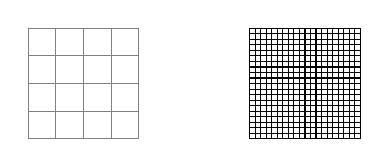
\begin{tikzpicture}[x=40pt,y=40pt]
    \draw[step=10pt,gray] (0,0) grid +(1,1);
    \draw[step=2pt]      (2,0) grid +(1,1);
  \end{tikzpicture}

  \medskip
  % Even though the left grid comes first in English reading order,
  % the right one is much more likely to be seen first: The
  % white-to-black contrast is higher than the gray-to-white
  % contrast. In addition, there are more ``places'' adding to the
  % overall contrast in the right grid.
  按照英文阅读顺序,应该先看到左边的网格,尽管如此,人们却更可能先看到右边的网格:
  黑白对比相较于灰白对比更加强烈,而且更多的“空间”增强了右边网格整体对比。

  % Things like grids and, more generally, help lines usually should not
  % grab the attention of the readers and, hence, should be typeset with
  % a low contrast to the background. Also, a loosely-spaced grid is
  % less distracting than a very closely-spaced grid.
  像网格或者是辅助线这样更普遍的东西,通常不应该分散读者的注意力。
  因此,排版这类内容时,同背景的对比应该弱一些。
  另外,稠密的网格比稀疏的网格更分散注意力。

\item
  % Dashed lines create many points at which there is black-to-white
  % contrast. Dashed or dotted lines can be very distracting and, hence,
  % should be avoided in general.
  虚线有很多点,形成了黑白对比。
  短划线或者点线可能很令人分神,因此一般避免使用。

  % Do not use different dashing patterns to differentiate curves in
  % plots. You lose data points this way and the eye is not
  % particularly good at ``grouping things according to a dashing
  % pattern.'' The eye is \emph{much} better at grouping things
  % according to colors.
  不要在作图中用不同类型的虚线样式来区分曲线。
  这种方式会丢失数据点,而且眼睛并不擅长“按照虚线样式划分事物”,而是更擅长按照颜色划分。
\item
  % Background patterns filling an area using  diagonal lines or
  % horizontal and vertical lines or just dots are almost always
  % distracting and, usually, serve no real purpose.
  用对角线、水平线、竖直线或者只是点形来填充背景,几乎总会令人分神,而且通常毫无用处。
\item
  % Background images and shadings distract and only seldomly add
  % anything of importance to a graphic.
  背景图片和渐变也令人分神,只能略微增加一些图形的重要性。
\item
  % Cute little clip arts can easily draw attention away from the
  % data.
  可爱的剪贴画很容易分散读者对数据的注意。
\end{itemize}
